\chapter{Technology of ice reservoirs}

AIRs are a natural evolution of Ladakh's agricultural system. They can be related to traditional water
harvesting technologies like the {\it zing}, which are small tanks where meltwater is collected through the use
of an intricate network of channels. The mountain oases of the Hindu Kush and Karakoram ranges
have similar irrigation networks \citep{nusserLocalKnowledgeGlobal2016}.

\begin{figure}[t]
\centering
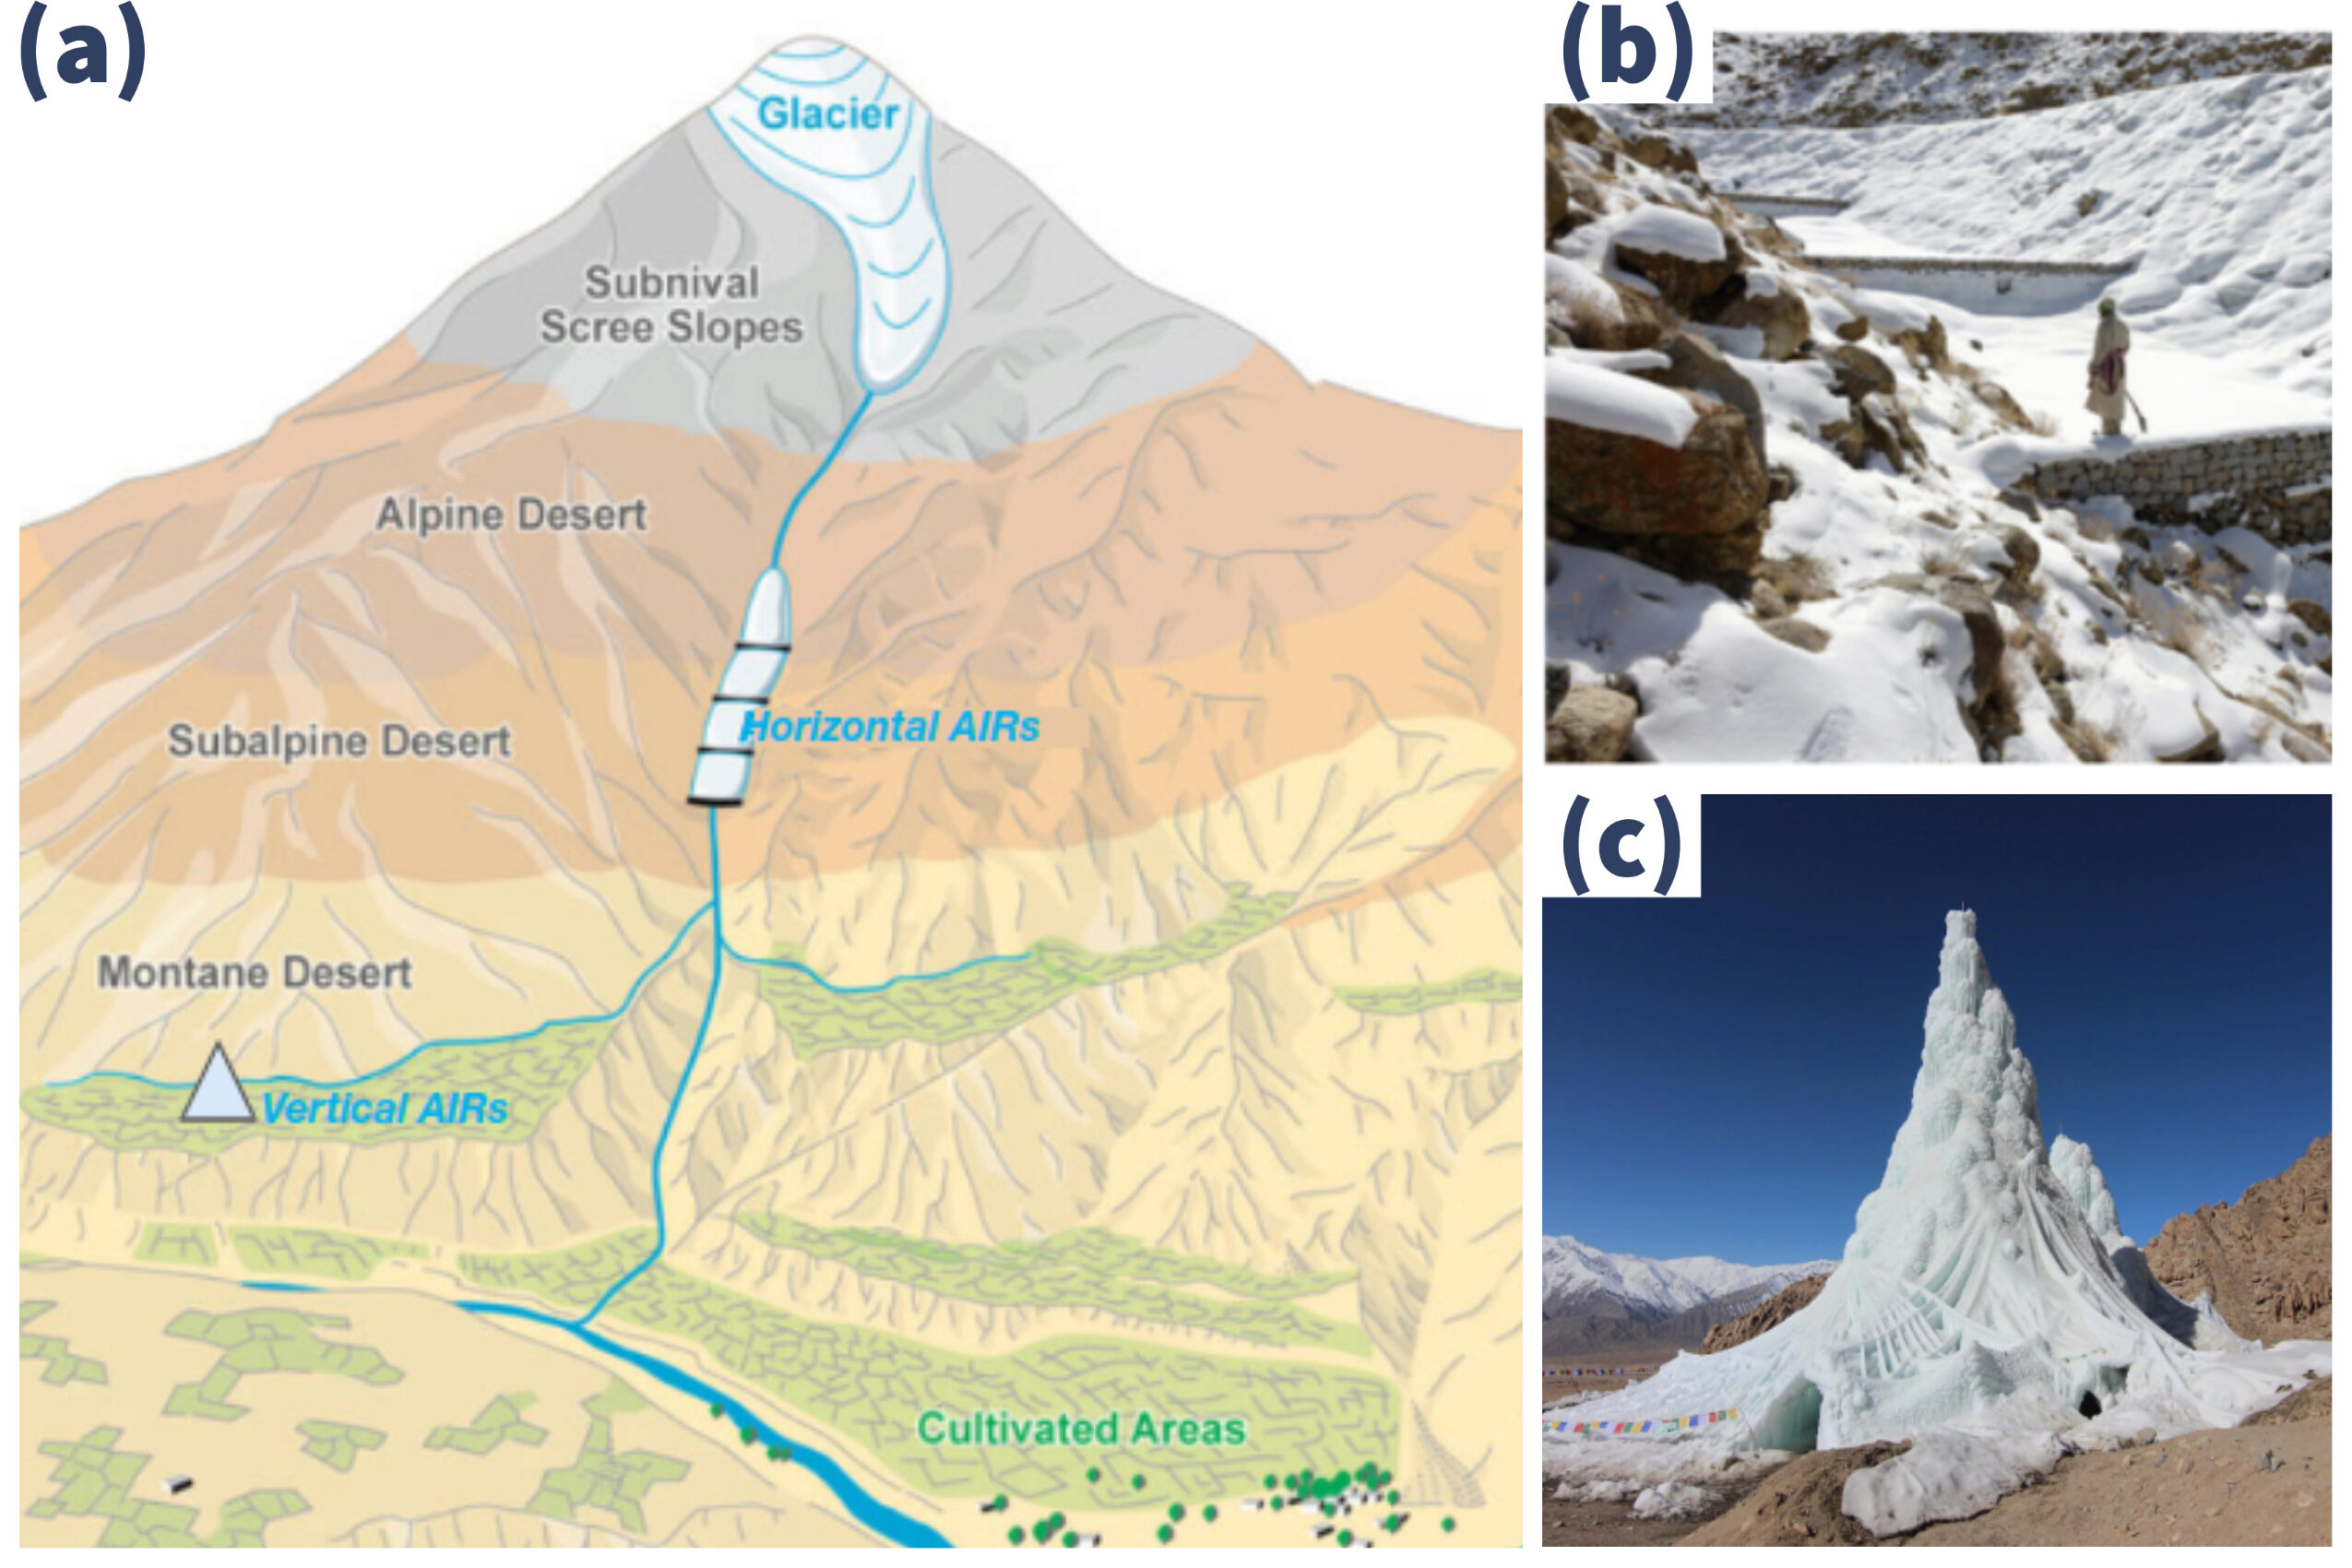
\includegraphics[width=12cm]{Figures/AIR_forms.jpg}

\caption{(a) Schematic overview of the position of artificial ice reservoirs. These constructions are located at
  altitudes between the glaciers and the irrigation networks in the cultivated areas. (b) Horizontal ice
  reservoirs at 3900 m, located above the village of Nang, Ladakh. The cascade is composed of a series of loose
  masonry walls ranging in height from 2 to 3 $m$, which help freeze water for storage. (c) Vertical ice
reservoirs at 3600 m, located above the village of Phyang, Ladakh. They are made using fountain systems. Adapted
from: \cite{nusserLocalKnowledgeGlobal2016}}

\label{fig:AIRforms}
\end{figure}

\section{Ice terraces}

\subsection{Invention}

Ice terraces are the oldest form of AIRs \citep{norphelArtificialGlacierHigh2009}. They used these irrigation
networks to amass a seasonal stock of ice by exploiting gravity and freezing winter temperatures. Chewang
Norphel, a well known engineer of the Leh Nutrition Project, introduced this innovation of local technology to
Ladakh in the 1980s and 1990s \citep{vinceGlacierMan2009}.

\subsection{Construction strategy}

These structures were built on south-facing slopes as a cascading series of rock walls in the river beds to
reduce runoff velocity and guide meltwater into shadowed areas (see Fig. \ref{fig:AIRforms}). The resulting
shallow pools begin to freeze as temperatures drop in winter, and ice accumulates. 

\subsection{Application}

\subsection{Drawbacks}

However, the location requirements and the construction cost of ice terraces were prohibitive for widespread
adoption. 


\section{Ice stupas}

\subsection{Innovation}

This prompted the invention of Ice stupas by Sonam Wangchuk in 2013 \ref{}. Due to their shape, Ice
stupas could be built adjacent to the irrigated plantations. It was also relatively cheaper. A typical Ice stupa
just requires a fountain nozzle mounted on a supply pipeline. The water source is usually a spring or a glacial
stream. Due to the altitude difference between the pipeline input and fountain output, water ejects from the
fountain nozzle as droplets that eventually lose their energy and accumulate as ice.  The fountain is manually
activated during the winter nights and is raised, through addition of metal pipes, when significant ice
accumulates below.

\subsection{Construction strategy}

\subsection{Application}

\subsection{Drawbacks}

\section{Improvement of construction strategies through weather-sensitive automation systems}

